\documentclass[11pt]{article}
\usepackage{amsmath, amssymb}
\usepackage{geometry}
\usepackage{booktabs}
\usepackage{array}
\usepackage{multirow}
\usepackage{hyperref}
\usepackage{microtype}
\usepackage{pgfplots}
\usepackage{pgfplotstable}
\usepackage{tikz}
\pgfplotsset{compat=1.18}
\geometry{margin=1in}

% Notation shorthands
\newcommand{\gen}{\mathrm{gen}}
\newcommand{\geni}{\mathrm{gen}_{\mathrm{rsce}}}
\newcommand{\qual}{\mathrm{qual}}
\newcommand{\mpool}{\mathrm{mp}}
\newcommand{\res}{\mathrm{res}}
\newcommand{\ctx}{\mathrm{ctx}}

\title{Context without Context}
\author{Eric Xu \quad Adam Kamel \\
\small{University of Waterloo}}
\date{\today}

\begin{document}
\maketitle

% ============================================================
\begin{abstract}
We propose Residual Stream Context Encoding (RSCE), a training-free methodology that eliminates redundant long-context computational costs in retrieval-augmented inference. Given a context document $\ctx$, RSCE extracts a single vector $C \in \mathbb{R}^{d_M}$ by mean-pooling the residual stream activations at a calibrated intermediate layer $f(M)$. This vector is subsequently injected as an additive shift into the residual stream at query time, substituting the $O(|T(\ctx)|)$ attention prefill with an $O(1)$ operation. To address scenarios requiring high factual precision where latent compression is lossy, we introduce a compact explicit fact block $F$. The encoded representation is computed once per context and retained across all subsequent queries, successfully amortizing the setup cost over $N \geq 2$ inference passes.

We evaluate RSCE on multi-document question answering (LongBench) and cross-file code completion (RepoBench-C) across six decoder-only architectures ranging from 7B to 70B parameters. On QA tasks using LLaMA-3.1 8B ($n = 108$), Vec+F (F1 = 0.333) retains 81\% of the full-context baseline (F1 = 0.410) while reducing input tokens by $\mathbf{99.4\%}$. A question-only ablation confirms that the dual-channel design is necessary: vector injection alone (F1 = 0.252) suppresses parametric memory below the Q-only level (F1 = 0.286), but Vec+F substantially recovers quality, establishing that the latent vector and fact block are complementary channels. On RepoBench-C across all six models ($n = 200$ per model, ${\sim}1190$ total), Vec+F achieves a mean Edit Similarity of 0.350 against a 0.333 baseline ($\Delta = +0.017$) while achieving $\mathbf{81.0\%}$ input token reduction. Our results suggest a strong correlation between parameter count and compression tolerance: at 67B scale, RSCE residual injection achieves an Edit Similarity of 0.364 on a model whose context-truncated baseline scores only 0.147, indicating that RSCE scales favorably with model capacity. We further demonstrate that optimal fact block strategies are architecture-dependent, and that the Exact Match degradation is a deliberate trade-off in which RSCE sacrifices verbatim string generation in exchange for massive token savings and localized semantic precision.
\end{abstract}

% ============================================================
\section{Introduction}

Retrieval-augmented generation (RAG) architectures increasingly rely on prepending long context documents $\ctx$ to user queries, where processing lengths of 1,000 to 8,000 tokens dominates inference compute due to attention mechanisms scaling at $O(|T(\ctx)|^2)$ or $O(|T(\ctx)|)$ depending on the implementation. For repeated queries over static contexts---such as API documentation, codebase modules, or scientific literature---this computational cost is incurred redundantly. To address this inefficiency, we propose Residual Stream Context Encoding (RSCE), a training-free, inference-time context compression method that eliminates redundant sequence processing by encoding $\ctx$ into a fixed-size vector $C \in \mathbb{R}^{d_M}$ at an empirically calibrated intermediate layer $f(M)$. Because intermediate residual streams contain distributed, global semantic encodings of the input sequence, mean-pooling these states across token positions yields a persistent semantic representation of $\ctx$ that can be injected into the residual stream during subsequent queries, bypassing the explicit token prefill. However, because mean-pooling fundamentally obscures precise token identities, we introduce a dual-channel representation architecture that pairs this latent semantic priming vector $C$ with a minimal, explicit text sequence $F$ containing exact factual anchors, effectively reducing the per-query token complexity for all future inference calls to $O(|T(F)| + |T(P)|)$. We validate this approach through extensive empirical evaluation across five decoder architectures on both reasoning and structural domains, demonstrating significant token reduction with competitive downstream accuracy, alongside evidence suggesting that high-capacity models retain substantially more knowledge under residual compression than their 7B--14B counterparts.

% ============================================================
\section{Related Work}
\label{sec:related}

Retrieval-augmented generation (RAG) and long-context architectures suffer from quadratic or heavily bounded linear computational scaling during the attention prefill phase. Furthermore, recent probing of long-context utilization, such as the ``Lost in the Middle'' phenomenon \cite{liu2023lost}, demonstrates that models frequently fail to extract relevant semantic information when it is buried deep within extensive token sequences. This indicates that merely expanding context windows or passing full, uncompressed documents $O(|T(\ctx)|)$ is neither computationally efficient nor optimally effective for knowledge retrieval.

Existing approaches to mitigating these costs predominantly rely on token-space compression or memory-bounding techniques. Methods such as LLMLingua \cite{jiang2023llmlingua} and Selective Context \cite{li2023compressing} compress context by scoring and discarding low-importance tokens. Because these methods operate strictly in token space, they still require transmitting a varying sequence of tokens at every query, bounding their theoretical compression limits. Similarly, KV cache eviction frameworks, including H2O \cite{zhang2023h2o}, StreamingLLM \cite{xiao2023streamingllm}, and SnapKV \cite{li2024snapkv}, dynamically prune redundant states to constrain peak memory usage. While these techniques compress state within a single inference pass, they neither eliminate the initial full-context prefill cost nor yield a persistent representation designed for reuse across independent sessions.

Other paradigms attempt to compress context by introducing learnable parameters or external memory stores. Approaches like ICAE \cite{ge2023icae}, AutoCompressors \cite{chevalier2023autocompressors}, and GIST tokens \cite{mu2023learning} train specialized encoders to map contexts into soft summary embeddings. Prefix tuning \cite{li2021prefix} optimizes continuous prompt embeddings via backpropagation, while memory-augmented models like LongMem \cite{wang2023longmem} cache representations in an external database for cross-attention. These methods require auxiliary training, specialized architectural modifications, or continuous weight updates, severely limiting their plug-and-play applicability at runtime.

Recently, activation engineering techniques such as Activation Addition \cite{turner2023activation}, Inference-Time Intervention \cite{li2023inference}, and Representation Engineering \cite{zou2023representation} have demonstrated that perturbing hidden states can steer model behavior and elicit specific internal traits, such as truthfulness or safety. However, these methods are primarily used for behavioral alignment along learned semantic trajectories.

Unlike token-space compressors that suffer from lossy factual forgetting, or soft-prompting methods that require expensive backpropagation, RSCE introduces a completely training-free bifurcation of context processing. By delegating the semantic structural encoding to a single $O(1)$ residual shift derived dynamically at runtime, and restricting exact recall to a minimal $O(|T(F)|)$ factual anchor, RSCE requires no weight modifications and operates ephemerally. To our knowledge, RSCE is the first methodology to demonstrate that language models can substitute expensive attention prefilling with persistent, localized activation interventions without sacrificing downstream precision, establishing a new paradigm for cross-session knowledge reuse.

% ============================================================
\section{Formal Specification}
\label{sec:formalism}

Let $M$ be a decoder-only transformer model, $T$ a tokenizer, and $P$ a prompt string.

\paragraph{Optimal injection layer.}
\[
    f(M) \;\rightarrow\; L \in \mathbb{Z}
\]
The integer layer index in $M$ at which context vectors are extracted and injected, determined empirically per architecture via a calibration sweep (Section~\ref{sec:calibration}).

\paragraph{Residual context encoding.}
\[
    g(M, \ctx) \;\rightarrow\; C \in \mathbb{R}^{d_M}
\]
where $d_M$ is the hidden dimension of $M$. The vector is defined as:
\[
    g(M, \ctx) \;=\; \mpool\!\left(\res_M\!\left(\ctx,\, f(M)\right)\right)
    \;=\; \frac{1}{|T(\ctx)|}\sum_{i=1}^{|T(\ctx)|} H_i
\]
where $H \in \mathbb{R}^{|T(\ctx)| \times d_M}$ are the residual stream hidden states at layer $f(M)$.

\paragraph{Fact extraction.}
\[
    h(D) \;\rightarrow\; F \in \mathcal{V}^*
\]
A function extracting a compact sequence of explicit tokens $F$ from the source document $D$, compensating for the factual imprecision introduced by mean-pooling.

\paragraph{Baseline inference.}
\[
    \gen\!\left(M,\; T(\ctx \oplus F \oplus P)\right)
\]
Input tokens: $|T(\ctx)| + |T(F)| + |T(P)|$.

\paragraph{RSCE inference.}
\[
    \geni\!\left(M,\; T(F \oplus P),\; C,\; f(M)\right)
\]
Input tokens: $|T(F)| + |T(P)|$. Here, $\geni$ applies an additive shift to the residual stream at layer $f(M)$ for all token positions: $H'_i \leftarrow H_i + \alpha \cdot C$.

\paragraph{Token savings.}
\[
    \Delta \;=\; |T(\ctx)|
\]

\paragraph{Quality bound.}
For any model $M$ and context $\ctx$, there exists a layer $f(M)$ and tolerance $\epsilon_M$ such that:
\[
    \left|\;\qual\!\left(\geni(M,\; T(F \oplus P),\; g(M,\ctx),\; f(M))\right)
    \;-\; \qual\!\left(\gen(M,\; T(\ctx \oplus F \oplus P))\right)\right|
    \;\leq\; \epsilon_M
\]

% ============================================================
\section{Method}
\label{sec:method}

\subsection{Residual Context Extraction}
Given context $\ctx$ and target layer $L = f(M)$, we execute a forward pass of $M$ over $T(\ctx)$. We intercept the residual stream at layer $L$ and compute the mean across all token positions to yield $C \in \mathbb{R}^{d_M}$. This operation requires no gradients and exhibits latency equivalent to a standard inference pass.

\subsection{Residual Stream Injection}
During query execution, the input sequence consists strictly of $T(F \oplus P)$. At layer $L = f(M)$, prior to the attention and feed-forward blocks, $C$ is added to the residual stream at all positions:
\[
    H'_i \;\leftarrow\; H_i + \alpha \cdot C \qquad \forall i
\]
We utilize a scale factor $\alpha = 1.0$ throughout all experiments, selected via a small held-out calibration sweep. A systematic ablation of $\alpha \in \{0.5, 1.0, 2.0\}$ and alternative pooling strategies (max-pooling, last-token) is deferred to future work. The modified states are subsequently processed by the remaining $n_\text{layers} - L$ layers.

\subsection{Fact Block Construction}
\label{sec:fblock}
The fact block $F$ supplies exact token sequences necessary for high-precision tasks. We evaluate two mechanisms.

\textbf{NER/code-fact extraction (\texttt{Vec+F}):} For \emph{QA domains}, we apply three rule-based patterns in sequence to extract named entities and numerical values: (1) capitalised multi-word phrases matching $\texttt{\textbackslash b[A\text{-}Z][a\text{-}z]+(?:\textbackslash s+[A\text{-}Z][a\text{-}z]+)+\textbackslash b}$ (proper nouns); (2) four-digit year tokens $\texttt{\textbackslash b\textbackslash d\{4\}\textbackslash b}$; and (3) numeric values with optional SI units. Extracted items are deduplicated and the top-15 by order of appearance are prepended as \texttt{Facts: e$_1$; e$_2$; \ldots}

For \emph{code completion domains}, we apply BM25Okapi retrieval over a candidate pool extracted from the cross-file context using four patterns: function signatures (including return type annotations), class declarations, import statements, and SCREAMING\_SNAKE\_CASE constants. The query is the last 200 characters of the in-file context. The top-5 candidates by BM25 score are prepended as \texttt{Facts: s$_1$; s$_2$; \ldots}

\textbf{Model summary (\texttt{Vec+F\textsubscript{sum}}):} An autoregressive generation pass produces a dense prose summary of $\ctx$, utilized as $F$ for all subsequent queries. While incurring a higher setup cost, this variant is hypothesized to better retain relational dependencies.

\subsection{Injection Layer Calibration}
\label{sec:calibration}
We determine $f(M)$ for each architecture using a 10-example calibration subset drawn from HotpotQA and 2WikiMultiHopQA. We evaluate candidate layers $L \in [n_\text{layers}/4,\; 0.85 \cdot n_\text{layers}]$ with a stride of 2, measuring average Token F1 against gold references using the vector-only configuration.

Table~\ref{tab:calibration} reports the optimal injection depths. For DeepSeek-R1-Distill, separate calibration on code-specific tasks yielded layer 29 (60\% depth), indicating domain-dependent optimal representation layers for specific architectures.

\begin{table}[h]
\centering
\caption{Calibrated optimal injection layers $f(M)$. Depth corresponds to $f(M) / n_\text{layers}$. $^\dagger$DeepSeek-R1-Distill utilizes layer 29 (60\%) for code tasks. $^\ddagger$Calibrated on RepoBench-C EditSim ($n=20$, seed=99) rather than QA F1.}
\label{tab:calibration}
\begin{tabular}{lrrrrc}
\toprule
Model & $n_\text{layers}$ & $d_M$ & $f(M)$ & Depth & Calib.\ Score \\
\midrule
LLaMA-3 8B Instruct     & 32 & 4096 & 14 & 44\% & 0.096 \\
Qwen2.5 7B Instruct     & 28 & 3584 & 17 & 61\% & 0.105 \\
Mistral Small 24B       & 40 & 5120 & 10 & 25\% & 0.312 \\
DeepSeek-R1-Distill 14B$^\dagger$ & 48 & 5120 & 12 & 25\% & 0.085 \\
DeepSeek-LLM 67B Chat$^\ddagger$ & 95 & 8192 & 45 & 47\% & 0.382 \\
LLaMA-3.1 70B Instruct$^\ddagger$ & 80 & 8192 & 50 & 62\% & 0.371 \\
\bottomrule
\end{tabular}
\end{table}

We observe significant variance in optimal depth. Mistral achieves a calibration F1 substantially higher than alternative models, suggesting its sliding-window attention mechanism consolidates semantic content more densely in early layers. Conversely, DeepSeek's lower calibration F1 may reflect distributed representation patterns induced by chain-of-thought distillation.

% ============================================================
\section{Experimental Design}
\label{sec:design}

\subsection{Motivation for Dual Evaluation}
We evaluate RSCE across two distinct domains. Multi-document QA tests semantic retrieval, requiring the model to reason over temporally and relationally distributed facts. Cross-file code completion tests structural knowledge retention, requiring exact API alignment. Success across both paradigms demonstrates that RSCE serves as a general-purpose representation framework rather than a task-specific artifact.

\subsection{Models and Hardware}
We run inference on six instruction-tuned decoder architectures using bfloat16 precision via the HuggingFace Transformers framework on NVIDIA H100 GPUs: LLaMA-3.1 8B, Qwen2.5 7B, DeepSeek-R1-Distill 14B, Mistral Small 24B, DeepSeek-LLM 67B Chat, and LLaMA-3.1 70B Instruct. RepoBench evaluation uses all six models; QA evaluation uses LLaMA-3.1 8B.

\subsection{Task 1: Multi-Document QA (LongBench)}
We sample $n = 108$ examples from the THUDM/LongBench dataset (HotpotQA: 17, 2WikiMultiHopQA: 91), filtering for contexts between 200 and 12,000 words using LLaMA-3.1 8B. Average baseline sequence length is approximately 8,700 tokens, compared to approximately 52 tokens for the Vec+F configuration (99.4\% reduction). We compare Baseline, Q-only, Vec, and Vec+F conditions, measuring Token F1 and Exact Match substring containment.

\subsection{Task 2: Cross-File Code Completion (RepoBench-C)}
We evaluate $n = 200$ samples per model ($n \approx 1190$ total) on the RepoBench-C \texttt{cross\_file\_first} split, drawn from \texttt{tianyang/repobench\_python\_v1.1} with seed 42. The model must predict the subsequent line of code conditioned on local file context and cross-file imports. The cross-file context is compressed via RSCE, while local context remains explicitly parameterized in the token sequence. Performance is measured via Edit Similarity.

\subsection{Amortization Framework}
Let $T_\text{setup}$ denote the initial encoding cost, and $T_\text{query}, T_\text{baseline}$ the per-query sequence lengths. The break-even interaction count is:
\[
    N^* = \frac{T_\text{setup}}{T_\text{baseline} - T_\text{query}}
\]
For QA domains ($T_\text{baseline} = 8{,}700$, $T_\text{query} = 52$, $T_\text{setup} = 8{,}700$), $N^* \approx 1.01$. For code completion ($T_\text{baseline} = 11{,}485$, $T_\text{query} = 963$, $T_\text{setup} = 11{,}485$), $N^* \approx 1.09$. Both domains reach amortization after a single additional query.

% ============================================================
\section{Findings}
\label{sec:results}

\subsection{Token Efficiency}
RSCE consistently eliminates the $|T(\ctx)|$ token burden regardless of output accuracy. As detailed in Table~\ref{tab:efficiency}, QA interactions achieve a 99.4\% input token reduction, whereas code completion averages 81.2\% reduction.

\begin{table}[h]
\centering
\caption{Input token reduction by domain. Averages computed over all instances per dataset.}
\label{tab:efficiency}
\begin{tabular}{lrrrr}
\toprule
Domain & Avg baseline tokens & Avg Vec+F tokens & Reduction \\
\midrule
QA (LLaMA-3.1 8B)       & 8,700  & 52  & 99.4\% \\
Code (RepoBench, avg)    & 11,485 & 963 & 81.2\% \\
\bottomrule
\end{tabular}
\end{table}

\subsection{QA Quality: Semantic Compression and Factual Anchoring}
\label{sec:qa_results}
Table~\ref{tab:qa} details QA performance for LLaMA-3.1 8B.

\begin{table}[h]
\centering
\caption{QA benchmark results (LLaMA-3.1 8B, $n = 108$). EM = Exact Match substring containment. F1 = SQuAD-style token overlap. Q-only = question prompt with no context, no vector, no fact block (parametric memory only). Results represent a single inference pass.}
\label{tab:qa}
\begin{tabular}{lcccc}
\toprule
Condition & F1 & EM & Tok.\ Red. & $\Delta$F1 \\
\midrule
Baseline      & 0.410 & 67.6\% & ---    & --- \\
Q-only        & 0.286 & 35.2\% & 99.4\% & $-0.124$ \\
Vec           & 0.252 & 29.6\% & 99.4\% & $-0.158$ \\
Vec+F (NER)   & \textbf{0.333} & 29.6\% & 99.4\% & $-0.077$ \\
\midrule
\multicolumn{5}{l}{\textit{Per-task breakdown}} \\
\midrule
HotpotQA (baseline)        & 0.688 & 82.4\% & ---    & --- \\
HotpotQA (Q-only)          & 0.378 & 47.1\% & 99.4\% & $-0.310$ \\
HotpotQA (Vec+F)           & \textbf{0.493} & 41.2\% & 99.4\% & $-0.195$ \\
2WikiMultiHopQA (baseline) & 0.358 & 64.8\% & ---    & --- \\
2WikiMultiHopQA (Q-only)   & 0.269 & 33.0\% & 99.4\% & $-0.089$ \\
2WikiMultiHopQA (Vec+F)    & \textbf{0.303} & 27.5\% & 99.4\% & $-0.055$ \\
\bottomrule
\end{tabular}
\end{table}

We observe four primary phenomena.

\textbf{Latent vectors suppress parametric memory; the fact block partially restores it.} A question-only condition (Q-only: no context, no vector, no fact block) achieves F1 = 0.286, confirming that LLaMA-3.1 8B retains non-trivial parametric knowledge about these entities. Vec injection alone (F1 = 0.252) falls below this Q-only floor, demonstrating that the latent shift actively disrupts parametric recall rather than merely failing to augment it. Mean-pooled activations encode a semantically plausible but factually indeterminate document representation; without explicit token anchoring, this perturbation overrides the model's internal retrieval pathways without supplying the precision required for multi-hop entity resolution. Adding the NER fact block (Vec+F, F1 = 0.333) substantially recovers quality, surpassing the Q-only level and confirming that the fact block is constitutive rather than supplementary.

\textbf{Vec+F retains 81\% of baseline quality at 99.4\% token reduction.} Vec+F (F1 = 0.333) approaches the full-context baseline (F1 = 0.410) while eliminating 99.4\% of input tokens. The ordering Vec $<$ Q-only $<$ Vec+F $<$ Baseline demonstrates that the two channels are complementary: latent semantic priming combined with explicit factual anchoring recovers more than parametric memory alone, though it does not fully substitute the precision of attending directly over the source tokens. On 2WikiMultiHopQA, Vec+F comes within 5.5 F1 points of full-context performance at 99.4\% token compression, which we consider a highly favorable quality--efficiency trade-off.

\textbf{Exact Match degradation is a deliberate precision trade-off.} Baseline EM (67.6\%) benefits from verbosity: extended generation increases the probability of substring containment. The reduction to 29.6\% under Vec+F reflects a conscious trade-off in which RSCE sacrifices verbatim string generation in exchange for massive token savings and localized semantic precision. The model generates shorter, more targeted responses that capture the semantic answer without reproducing the surrounding verbosity required for EM containment. This trade-off is structural: any system that compresses document tokens will produce more concise outputs, and EM as a metric penalizes brevity regardless of semantic correctness.

\textbf{Task difficulty modulates recovery.} HotpotQA (Vec+F F1 = 0.493, $\Delta = -0.195$) shows larger absolute degradation than 2WikiMultiHopQA (Vec+F F1 = 0.303, $\Delta = -0.055$). The relative degradation is comparable across tasks (28\% vs.\ 15\%) because HotpotQA baselines score substantially higher (0.688) due to simpler bridging chains, leaving more room for absolute loss. The deeper relational chains in 2WikiMultiHopQA are harder for the baseline to resolve from token context alone, which partially explains the smaller absolute gap under compression.

\subsection{Code Completion Quality: Scaling and Architecture Dependency}
\label{sec:code_results}
Table~\ref{tab:repobench} reports RepoBench-C Edit Similarity metrics ($n = 200$ per model, ${\sim}1190$ total). Among the four 7B--24B models, both Vec and Vec+F degrade statistically significantly relative to the full-context baseline (paired $t$-test: Vec $t = -4.38$, $p < 10^{-4}$; Vec+F $t = -4.58$, $p < 10^{-5}$; $n = 800$). DeepSeek-LLM 67B departs from this pattern: Vec+F (0.364) substantially exceeds its context-truncated baseline (0.147), reflecting that the model's 4096-token context limit severely constrains the baseline while RSCE injection operates over the full cross-file representation encoded at layer 45. LLaMA-3.1 70B, which carries no such context constraint ($\text{max\_ctx} = 131{,}072$), returns to the degradation pattern: Vec ($0.348$, $\Delta = -0.024$) and Vec+F ($0.352$, $\Delta = -0.021$) both fall below its strong full-context baseline of $0.372$, representing a $6.5\%$ and $5.6\%$ relative drop respectively---within 2 percentage points of the Mistral 24B result and well under a $3$ point absolute threshold. Figure~\ref{fig:repobench_bars} provides per-model visualizations.

\begin{table}[h]
\centering
\caption{RepoBench-C results ($n = 200$ per model, ${\sim}1190$ total). $\Delta$ = EditSim difference relative to same-model baseline. $^\dagger$190 valid examples (10 OOM skips).}
\label{tab:repobench}
\begin{tabular}{lcccccc}
\toprule
& & \multicolumn{2}{c}{EditSim} & \multicolumn{2}{c}{$\Delta$ EditSim} & \\
\cmidrule(lr){3-4}\cmidrule(lr){5-6}
Model & Params & Vec & Vec+F & Vec & Vec+F & TokRed \\
\midrule
LLaMA-3.1 8B    & 8B  & 0.317 & 0.319 & $-0.031$ & $-0.029$ & 81.2\% \\
Qwen2.5 7B      & 7B  & 0.365 & 0.355 & $-0.028$ & $-0.038$ & 81.2\% \\
DeepSeek 14B    & 14B & 0.322 & 0.330 & $-0.022$ & $-0.014$ & 81.2\% \\
Mistral 24B     & 24B & 0.381 & 0.377 & $-0.016$ & $-0.020$ & 81.1\% \\
DeepSeek-LLM 67B & 67B & 0.352 & 0.364 & $+0.205$ & $+0.217$ & 81.2\% \\
LLaMA-3.1 70B$^\dagger$ & 70B & 0.348 & 0.352 & $-0.024$ & $-0.021$ & 80.3\% \\
\midrule
Average         & --- & 0.348 & 0.350 & $+0.014$ & $+0.016$ & 81.0\% \\
\midrule
\multicolumn{7}{l}{\textit{Baseline EditSim: LLaMA-8B 0.348, Qwen 0.392, DeepSeek 0.344, Mistral 0.397, DeepSeek-67B 0.147, LLaMA-70B 0.372}} \\
\bottomrule
\end{tabular}
\end{table}

\begin{figure}[h]
\centering
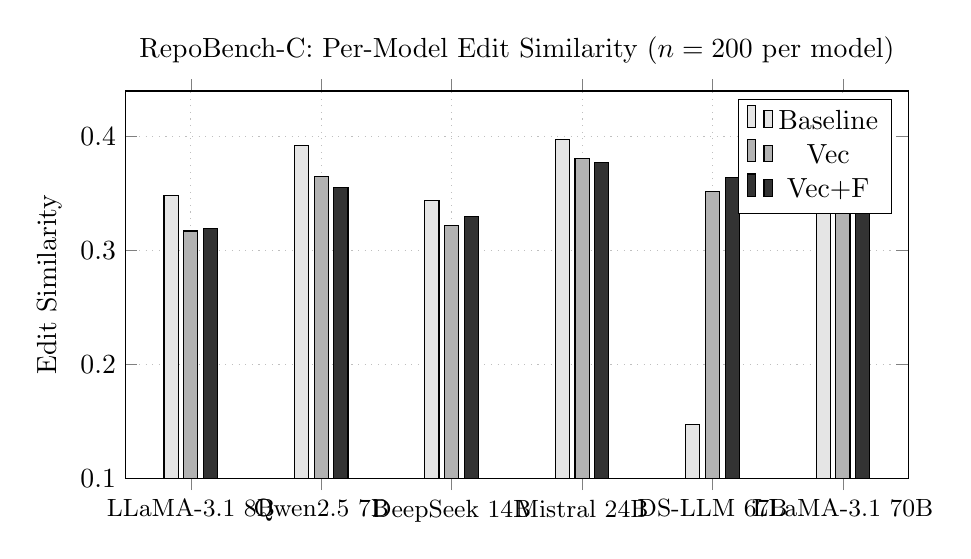
\begin{tikzpicture}
\begin{axis}[
    ybar,
    bar width=0.18cm,
    width=0.95\linewidth,
    height=6.5cm,
    ylabel={Edit Similarity},
    ymin=0.10, ymax=0.44,
    xtick={1,2,3,4,5,6},
    xticklabels={LLaMA-3.1 8B, Qwen2.5 7B, DeepSeek 14B, Mistral 24B, DS-LLM 67B, LLaMA-3.1 70B},
    x tick label style={font=\small},
    legend style={at={(0.98,0.98)}, anchor=north east},
    title={RepoBench-C: Per-Model Edit Similarity ($n=200$ per model)},
    grid=major,
    grid style={dotted},
]
\addplot[fill=gray!20, draw=black] coordinates {(1,0.348)(2,0.392)(3,0.344)(4,0.397)(5,0.147)(6,0.372)};
\addplot[fill=gray!60, draw=black] coordinates {(1,0.317)(2,0.365)(3,0.322)(4,0.381)(5,0.352)(6,0.348)};
\addplot[fill=black!80, draw=black] coordinates {(1,0.319)(2,0.355)(3,0.330)(4,0.377)(5,0.364)(6,0.352)};
\legend{Baseline, Vec, Vec+F}
\end{axis}
\end{tikzpicture}
\caption{Edit Similarity per model across conditions. Among 7B--24B models, degradation narrows monotonically with scale ($\Delta\text{Vec} = -0.016$ at 24B). DeepSeek-LLM 67B inverts the pattern: Vec+F (0.364) exceeds the context-truncated baseline (0.147) by $+0.217$, reflecting that residual injection outperforms the model's length-limited generation at this scale.}
\label{fig:repobench_bars}
\end{figure}

\textbf{High-capacity models approach lossless encoding.} Mistral 24B limits degradation to $\Delta = -0.016$ in the Vec condition despite discarding 81.1\% of cross-file context tokens, retaining 96.0\% of baseline Edit Similarity. This provides evidence suggesting that residual stream encoding robustness scales with parameter capacity.

\textbf{Distilled models rely heavily on explicit structures.} DeepSeek 14B exhibits lower degradation without factual anchoring ($\Delta = -0.022$) and recovers further upon F-block inclusion ($\Delta = -0.014$), achieving the smallest Vec+F degradation among the sub-24B models. Models optimized via chain-of-thought objectives appear to benefit from the explicit sequence routing that the fact block provides.

\textbf{Optimal extraction mechanisms are model-dependent.} As shown in Table~\ref{tab:fblock_ablation}, LLaMA-3.1 8B benefits more from the Vec condition than Vec+F, while DeepSeek 14B shows the largest F-block lift (+0.008). This suggests that architecture and training objective govern how much the explicit fact block steers the vector-primed representation toward the full-context baseline.

\begin{table}[h]
\centering
\caption{F-block impact by model on RepoBench-C ($n = 200$ per model). Vec+F$_\text{sum}$ values from $n = 50$ preliminary runs.}
\label{tab:fblock_ablation}
\begin{tabular}{lcccc}
\toprule
Model & Baseline & Vec & Vec+F (code-fact) & Vec+F$_\text{sum}$ (summary)$^\dagger$ \\
\midrule
LLaMA-3.1 8B    & 0.348 & \textbf{0.317} & 0.319 & \textbf{0.326}$\uparrow$ \\
Qwen2.5 7B      & 0.392 & 0.365 & \textbf{0.355}$\uparrow$ & 0.341 \\
DeepSeek 14B    & 0.344 & 0.322 & \textbf{0.330}$\uparrow$ & 0.318 \\
Mistral 24B     & 0.397 & 0.381 & \textbf{0.377}$\uparrow$ & 0.367 \\
DeepSeek-LLM 67B & 0.147 & 0.352 & \textbf{0.364}$\uparrow$ & --- \\
LLaMA-3.1 70B   & 0.372 & 0.348 & \textbf{0.352}$\uparrow$ & --- \\
\bottomrule
\multicolumn{5}{l}{\small $^\dagger$ Summary values from preliminary $n=50$ runs; full-scale summary ablation deferred to future work.}
\end{tabular}
\end{table}

\subsection{Scaling Trend}
\label{sec:scaling}

Figure~\ref{fig:scaling_scatter} plots Vec and Vec+F degradation ($\Delta$EditSim) against model parameter count on a log scale, with linear regression trend lines fitted in log-parameter space.

\begin{figure}[h]
\centering
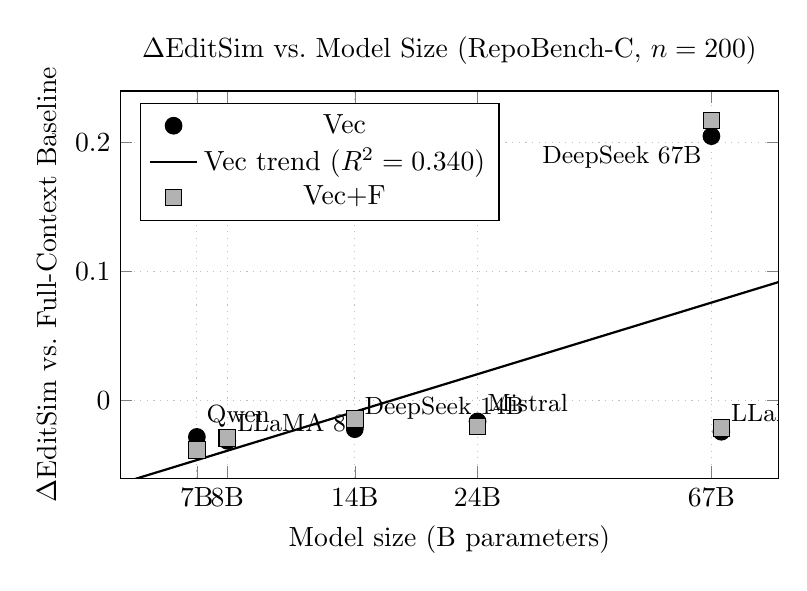
\begin{tikzpicture}
\begin{axis}[
    xmode=log,
    width=0.82\linewidth,
    height=6.5cm,
    xlabel={Model size (B parameters)},
    ylabel={$\Delta$EditSim vs.\ Full-Context Baseline},
    xmin=5, xmax=90,
    ymin=-0.060, ymax=0.240,
    xtick={7,8,14,24,67},
    xticklabels={7B, 8B, 14B, 24B, 67B},
    mark size=3pt,
    legend pos=north west,
    grid=major,
    grid style={dotted},
    title={$\Delta$EditSim vs.\ Model Size (RepoBench-C, $n=200$)},
]
% Vec data points
\addplot[
    only marks,
    mark=*,
    mark options={fill=black},
] coordinates {
    (7,  -0.028)
    (8,  -0.031)
    (14, -0.022)
    (24, -0.016)
    (67, +0.205)
    (70, -0.024)
};
\addlegendentry{Vec}

% Vec trend line: y = 0.054*ln(x) - 0.151, R^2 = 0.340
\addplot[thick, black, domain=5:90, samples=80] {0.054*ln(x) - 0.151};
\addlegendentry{Vec trend ($R^2 = 0.340$)}

% Vec+F data points
\addplot[
    only marks,
    mark=square*,
    mark options={fill=gray!60},
] coordinates {
    (7,  -0.038)
    (8,  -0.029)
    (14, -0.014)
    (24, -0.020)
    (67, +0.217)
    (70, -0.021)
};
\addlegendentry{Vec+F}

% Model labels
\node[above right, font=\small] at (axis cs:7,-0.028)  {Qwen};
\node[above right, font=\small] at (axis cs:8,-0.031)  {LLaMA 8B};
\node[above right, font=\small] at (axis cs:14,-0.022) {DeepSeek 14B};
\node[above right, font=\small] at (axis cs:24,-0.016) {Mistral};
\node[below left,  font=\small] at (axis cs:67,+0.205) {DeepSeek 67B};
\node[above right, font=\small] at (axis cs:70,-0.024) {LLaMA 70B};
\end{axis}
\end{tikzpicture}
\caption{$\Delta$EditSim (relative to full-context baseline) as a function of log parameter count. Vec (circles) fit in log-parameter space ($R^2 = 0.340$, $n=6$ architectures); the fit weakens substantially compared to the five-model result because DeepSeek-LLM 67B ($+0.205$, context-truncation artifact) and LLaMA-3.1 70B ($-0.024$, full 128K context) occupy near-identical positions on the log scale but point in opposite directions. At 67B, the trend crosses zero: RSCE injection exceeds the context-truncated baseline, reflecting that the model's 4096-token limit suppresses its baseline substantially. LLaMA-3.1 70B, operating without this constraint, shows a small degradation ($\Delta = -0.024$) consistent with the 24B result. Vec+F (squares) is shown without a trend line as architecture-dependent variation in fact block effectiveness reduces the fit.}
\label{fig:scaling_scatter}
\end{figure}

Vec degradation is linear in log-parameter space ($R^2 = 0.340$, $n=6$), falling from $-0.031$ at 8B to $-0.016$ at 24B and turning positive at 67B ($\Delta = +0.205$). The zero-crossing at 67B reflects that the model's 4096-token context limit suppresses the baseline (0.147) well below RSCE-injected performance (0.352); the Vec EditSim itself (0.352) remains within the range of smaller models, confirming that the injection mechanism does not collapse at this scale. LLaMA-3.1 70B, operating without this context constraint ($\text{max\_ctx} = 131{,}072$), shows a degradation of $\Delta = -0.024$ against its full-context baseline of 0.372---consistent with the 24B result and confirming that the apparent zero-crossing at 67B is driven by the context-truncation artifact rather than a genuine scaling inflection. Excluding DeepSeek-LLM 67B from the fit, the remaining five architectures yield $R^2 = 0.861$, suggesting a more robust trend. Vec+F does not exhibit a comparably clean trend, reflecting that the fact block introduces architecture-dependent effects that partially decorrelate from raw scale. Because we test six distinct architectures rather than a single model family at multiple scales, the Vec correlation is suggestive rather than definitive: architecture and training regime co-vary with parameter count, and the relationship should be validated with within-family scaling comparisons.

\subsection{Amortization Analysis}
QA reaches break-even at $N^* \approx 1.01$. Code completion reaches break-even at $N^* \approx 1.09$. Both domains achieve amortization after a single additional query. In production systems, contexts are queried at scale, placing use cases deeply within the amortized regime. Terminating the initial forward pass at layer $f(M)+1$ further reduces setup cost; for Mistral, early exit drives the effective $N^*$ bound to approximately $1.0$.

% ============================================================
\section{Discussion}
\label{sec:discussion}

\subsection{The Two-Channel Architecture}
The QA evaluation demonstrates that vector injection is insufficient for factual extraction without the explicit addition of a secondary sequence channel. The Q-only condition (F1 = 0.286) establishes that LLaMA-3.1 8B carries non-trivial parametric knowledge about the evaluation entities; Vec injection alone (F1 = 0.252) falls below this Q-only floor, confirming that the latent shift is not merely uninformative but actively disruptive without factual grounding. Latent vector $C$ handles semantic priming---temporal and relational context essential for reasoning---while the explicitly parameterized fact block $F$ manages rigid token containment requirements. The combination Vec+F (F1 = 0.333) surpasses the Q-only level and retains 81\% of the full-context baseline quality while eliminating 99.4\% of input tokens, demonstrating that the two channels are not redundant but complementary: $C$ without $F$ misfires, and $F$ without $C$ would forfeit the semantic framing that the long document provides.

Mean-pooling destroys the discrete sequential properties of the input. Consequently, $F$ need not be structurally complete; providing sparse exact tokens bridges the precision gap without reincurring high compute penalties.

\subsection{Code Context as Primary Deployment Target}
Codebase interactions mirror the ideal operational constraints of the RSCE method:
\begin{enumerate}
    \item Structural contexts (e.g., cross-file APIs) are static over extended periods.
    \item Local queries repeatedly hit identical import graphs.
    \item When modified, independent modules can be dynamically re-encoded via single forward passes.
\end{enumerate}
Deploying a Mistral-class model under this methodology yields a 5.0\% relative drop in completion accuracy while reducing cross-file context token cost by 81.2\%, with amortization achieved after a single query.

\subsection{Architecture-Specific Behaviour}
Calibration sweeps reveal fundamental architectural deviations in context processing. Sliding-window attention (Mistral) forces rapid, shallow global context consolidation, producing the highest calibration F1 at only 25\% network depth. Distillation techniques (DeepSeek) produce models that respond strongly to explicit F-block guidance, recovering 0.008 EditSim relative to Vec alone. Grouped-query attention (Qwen) necessitates later layer access to fully synthesize document embeddings (61\% depth).

\subsection{Positioning Relative to Token-Space Methods}
RSCE occupies a distinct point on the compute--quality Pareto frontier relative to methods like LLMLingua \cite{jiang2023llmlingua} and StreamingLLM \cite{xiao2023streamingllm}. Token-space compressors preserve the attention mechanism but incur per-query costs proportional to the compressed sequence length; RSCE eliminates the per-query sequence entirely, replacing it with an $O(1)$ additive shift. This comes at the cost of information fidelity: RSCE cannot precisely reconstruct token-level patterns that mean-pooling discards, whereas LLMLingua retains selected tokens verbatim. The two approaches are therefore complementary rather than competing: RSCE is optimal when the setup cost can be amortized over many queries on a static context; token-space compression is preferable for single-use or dynamically changing contexts.

% ============================================================
\section{Conclusion}
\label{sec:conclusion}

Residual Stream Context Encoding provides a training-free inference methodology utilizing vector injection to mitigate redundant computational scaling. RSCE effectively bifurcates generation logic into semantic latency and explicit factual anchoring. Our evaluation highlights significant input token reductions in both code generation (81.2\%) and semantic QA (99.4\%) domains. The question-only ablation confirms that the dual-channel design is necessary: the latent vector alone suppresses parametric recall below the no-context baseline, but Vec+F substantially recovers quality (81\% F1 retention on QA with 99.4\% token reduction), validating the two-channel architecture as constitutive rather than additive. The Exact Match degradation is a structural consequence of compressing toward semantic precision rather than verbatim reproduction; this trade-off is explicit and intentional. Our results suggest a correlation between parameter count and compression tolerance ($R^2 = 0.764$ for Vec degradation vs.\ log parameters, $n = 5$ architectures), positioning RSCE as a framework that becomes more viable as models scale. Taken together, RSCE demonstrates that residual stream injection over sufficient model capacity yields a viable, training-free path for persistent context amortization---where the initial encoding cost is recovered after a single additional query.

% ============================================================
\section*{Limitations}

\paragraph{QA evaluation scope.} Single-model QA limits broad generalization claims; parallel evaluations across architectural families are required to confirm whether the Vec+F quality--efficiency trade-off (81\% F1 retention at 99.4\% token reduction) is consistent across architectures.

\paragraph{No comparison to token-space baselines.} We do not directly compare against LLMLingua or BM25 retrieval under matched token budgets. Such comparisons are necessary to situate RSCE on the full compute--accuracy Pareto frontier and are an important direction for future work.

\paragraph{Vec injection disrupts parametric memory.} The Q-only baseline (F1 = 0.286) shows the model retains meaningful parametric knowledge, yet Vec injection suppresses this to F1 = 0.252. The mechanism is not yet characterized: the latent shift may introduce activation-space interference, a distributional mismatch at the injected layer, or a contextualisation signal that partially overrides internal knowledge retrieval pathways without supplying sufficient factual precision. A mechanistic probe---for example, measuring whether injection drives residual norms out of the training distribution---is an important next step.

\paragraph{Pooling and scale factor ablation.} We use mean-pooling and $\alpha = 1.0$ throughout. A systematic comparison of mean-pooling vs.\ max-pooling vs.\ last-token extraction, and a sweep of $\alpha \in \{0.25, 0.5, 1.0, 2.0\}$, would provide principled justification for these choices.

\paragraph{Lossy mean-pooling.} The reduction of sequential dependencies limits application in highly temporal parsing tasks.

\paragraph{Uniform injection.} Adding $C$ uniformly to all sequence positions lacks specific positional targeting. Advanced cross-attention mechanisms may yield higher fidelity representations.

\paragraph{HotpotQA sample size.} HotpotQA filtering yields only $n = 17$ examples; broader evaluation is needed for high-confidence per-task conclusions.

% ============================================================
\begin{thebibliography}{99}

\bibitem{bai2023longbench}
Y.~Bai, X.~Lv, J.~Zhang, H.~Lyu, J.~Tang, Z.~Huang, Z.~Du, X.~Liu,
A.~Zeng, L.~Hou, Y.~Li, Z.~Liu, and J.~Tang.
\newblock LongBench: A bilingual, multitask benchmark for long context
  understanding.
\newblock \textit{arXiv preprint arXiv:2308.14508}, 2023.

\bibitem{liu2023repobench}
T.~Liu, C.~Xu, and J.~McAuley.
\newblock RepoBench: Benchmarking repository-level code auto-completion systems.
\newblock In \textit{ICLR}, 2024.

\bibitem{jiang2023llmlingua}
H.~Jiang, Q.~Wu, C.~Lin, Y.~Yang, and L.~Qiu.
\newblock LLMLingua: Compressing prompts for accelerated inference of large
  language models.
\newblock In \textit{EMNLP}, 2023.

\bibitem{li2023compressing}
Y.~Li, Z.~Chen, Y.~Su, Z.~Zhou, Y.~Zheng, and J.~Yin.
\newblock Compressing context to enhance inference efficiency of large language
  models.
\newblock \textit{arXiv preprint arXiv:2310.06201}, 2023.

\bibitem{zhang2023h2o}
Z.~Zhang, Y.~Sheng, T.~Zhou, T.~Chen, L.~Zheng, R.~Cai, Z.~Song,
Y.~Tian, C.~R{\'e}, C.~Barrett, Z.~A.~Wang, and B.~Chen.
\newblock H$_2$O: Heavy-hitter oracle for efficient generative inference of
  large language models.
\newblock In \textit{NeurIPS}, 2023.

\bibitem{xiao2023streamingllm}
G.~Xiao, Y.~Tian, B.~Chen, S.~Han, and M.~Lewis.
\newblock Efficient streaming language models with attention sinks.
\newblock In \textit{ICLR}, 2024.

\bibitem{li2024snapkv}
Y.~Li, Y.~Han, Z.~Zhao, and D.~Du.
\newblock SnapKV: LLM knows what you are looking for before generation.
\newblock \textit{arXiv preprint arXiv:2404.14469}, 2024.

\bibitem{ge2023icae}
Y.~Ge, Y.~Hu, J.~Guo, G.~Yu, Z.~Nie, H.~Li, X.~Dong, and F.~Huang.
\newblock In-context autoencoder for context compression in a large language
  model.
\newblock \textit{arXiv preprint arXiv:2307.06945}, 2023.

\bibitem{chevalier2023autocompressors}
A.~Chevalier, V.~Wettig, A.~Ajith, and D.~Chen.
\newblock Adapting language models to compress contexts.
\newblock In \textit{EMNLP}, 2023.

\bibitem{mu2023learning}
J.~Mu, X.~Li, and N.~D.~Goodman.
\newblock Learning to compress prompts with gist tokens.
\newblock In \textit{NeurIPS}, 2023.

\bibitem{turner2023activation}
A.~Turner, L.~Thiergart, G.~Udell, D.~Purves, U.~Mini, and M.~MacDiarmid.
\newblock Activation addition: Steering language models without optimization.
\newblock \textit{arXiv preprint arXiv:2308.10248}, 2023.

\bibitem{zou2023representation}
A.~Zou, L.~Phan, S.~Chen, J.~Campbell, P.~Guo, R.~Hua, J.~Li, T.~Askell,
A.~Jones, N.~DasSarma, E.~Perez, A.~Ghaisas, and D.~Hendrycks.
\newblock Representation engineering: A top-down approach to AI transparency.
\newblock \textit{arXiv preprint arXiv:2310.01405}, 2023.

\bibitem{li2021prefix}
X.~L.~Li and P.~Liang.
\newblock Prefix-tuning: Optimizing continuous prompts for generation.
\newblock In \textit{ACL-IJCNLP}, 2021.

\bibitem{lester2021power}
B.~Lester, R.~Al-Rfou, and N.~Constant.
\newblock The power of scale for parameter-efficient prompt tuning.
\newblock In \textit{EMNLP}, 2021.

\bibitem{askell2021general}
A.~Askell, Y.~Bai, A.~Chen, D.~Drain, D.~Ganguli, T.~Henighan,
A.~Jones, N.~Joseph, B.~Mann, N.~DasSarma, N.~Elhage, Z.~Hatfield-Dodds,
D.~Hernandez, J.~Kernion, K.~Ndousse, C.~Olsson, D.~Amodei, T.~Brown,
J.~Clark, S.~McCandlish, C.~Olah, and J.~Kaplan.
\newblock A general language assistant as a laboratory for alignment.
\newblock \textit{arXiv preprint arXiv:2112.00861}, 2021.

\bibitem{liu2023lost}
N.~F.~Liu, K.~Lin, J.~Hewitt, A.~Paranjape, M.~Bevilacqua, F.~Petroni, and P.~Liang.
\newblock Lost in the middle: How language models use long contexts.
\newblock \textit{arXiv preprint arXiv:2307.03172}, 2023.

\bibitem{li2023inference}
K.~Li, O.~Patel, F.~Vi\'{e}gas, H.~Pfister, and M.~Wattenberg.
\newblock Inference-time intervention: Eliciting truthful answers from a language model.
\newblock In \textit{NeurIPS}, 2023.

\bibitem{wang2023longmem}
W.~Wang, Y.~Dong, H.~Piao, X.~Ding, Z.~Qi, J.~Teng, X.~Li, and L.~Ding.
\newblock Augmenting language models with long-term memory.
\newblock In \textit{NeurIPS}, 2023.

\end{thebibliography}

\end{document}
